%------------------------------------------------------------------------------------------------------------------------
\chapter{現行ピクセルモジュールの電荷較正}
\label{sec:chap3}
%------------------------------------------------------------------------------------------------------------------------

FEチップから得られるToT(Time over Threshold)を荷電粒子がシリコンセンサーに落とす電荷に較正する必要がある。本章では、電荷較正のための試験電荷生成回路の詳細について説明し、その後に電荷較正手法について述べる。

%------------------------------------------------------------------------------------------------------------------------
\section{試験電荷生成回路}
\label{sec:analog}
%------------------------------------------------------------------------------------------------------------------------
\fref{fig:analog}に試験電荷生成回路の概略図を示す。センサーにおいて生成された電子をFEチップにおいて検知するために、バンプにより接合されている。内部電位によりバンプに向かってドリフトした電子を検出し、バンプの接合部からFEチップへ送り、その信号をToTにデジタル変換し、後段のフレキシブル基板へ信号を送る。

一方で、Thresholdの測定や電荷較正のために用いる電荷はFEチップ内の回路で生成する。FEチップにおいて試験電荷を生成するために、電圧$V_\mathrm{cal}$を自由に設定できる回路と2つのキャパシタ$C_\mathrm{low}, C_\mathrm{high}$が搭載されている。試験電荷生成のために、$C_\mathrm{low}=8\ \si{fF}$のキャパシタを用いる場合と、$C_\mathrm{low}+C_\mathrm{high}=40\ \si{fF}$の合成キャパシタを用いる場合がある。$C_\mathrm{low}+C_\mathrm{high}$の合成キャパシタを用いる場合は生成した試験電荷から得られるToTが約$10\%$小さく出力されることがわかっている。そのため、Thresholdの測定や電荷較正を行う際には、$C_\mathrm{low}$のキャパシタを用いて試験電荷の生成を行う。

\begin{figure}[tbp]
  \centering
  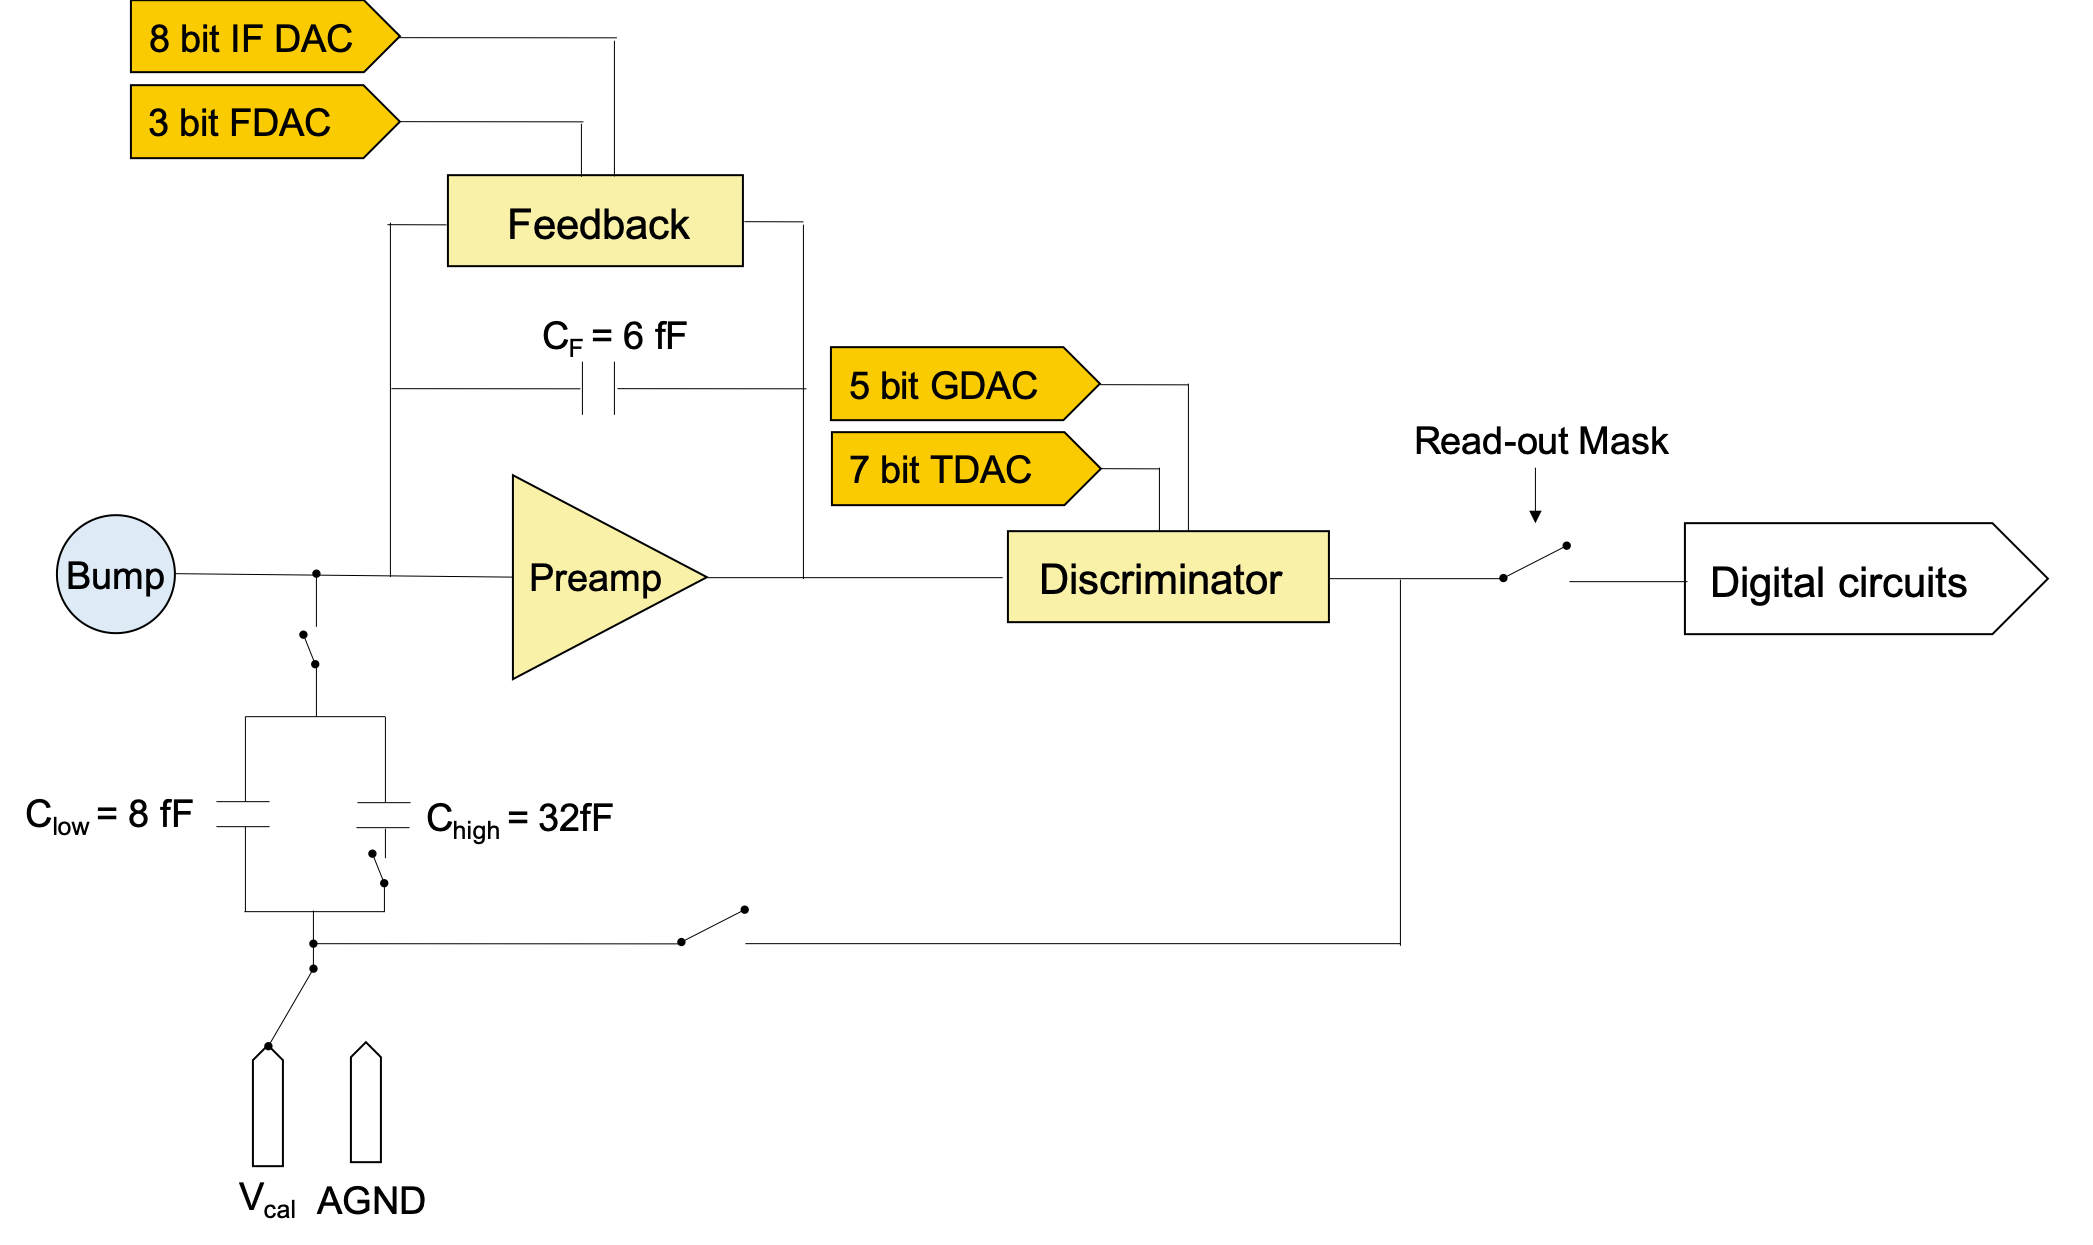
\includegraphics[height=7cm,keepaspectratio]{analog2.png}
  \caption[試験電荷生成回路の概略図]{試験電荷生成回路の概略図。電荷較正やThresholdスキャンのための試験電荷は$V_\mathrm{cal}$とキャパシタの組み合わせによって生成される。}
  \label{fig:analog}
\end{figure}


%------------------------------------------------------------------------------------------------------------------------
\section{電荷較正手法}
\label{sec:calibway}
%------------------------------------------------------------------------------------------------------------------------
ピクセルモジュールの出力であるToTを較正し、荷電粒子が落とした電荷量に変換する方法について説明する。各ピクセル間の差異を少なくするために、ToTの較正を行う前に、ThresholdやToTを目標値になるようチューニングを行う必要がある。以下ではチューニングと電荷較正の方法について説明する。


%------------------------------------------------------------------------------------------------------------------------
\subsection{チューニング}
\label{sec:tuning}
%------------------------------------------------------------------------------------------------------------------------
各ピクセルにおけるThresholdと、ある基準電荷量の信号に対するToTを任意の値に調整するためにFEチップのチューニングを行う。RUN2におけるThresholdおよび任意の値に対するToTの目標値をそれぞれ\tref{tab:thresholdtuning}、\tref{tab:tottuning}に示す。さらに、2022年3月から始まるRUN3では、B-LayerのThresholdは$3500\ \si{e}$でありToTのチューニングは$20\ \si{ke}$の電荷に対して$18\ \si{ToT}$、IBLのThresholdは$1500\ \si{e}$でありToTのチューニングは$16\ \si{ke}$の電荷に対して$10\ \si{ToT}$である。

\begin{table}[tbp]
  \begin{center}
    \caption[各LayerにおけるThresholdの値]{各LayerにおけるThresholdの目標値。}
    \label{tab:thresholdtuning}
    \begin{tabular}{|l||r|r|r|r|}
    \hline
      Layer名  & 2015年($4\ \si{fb^{-1}}$) & 2016年($39\ \si{fb^{-1}}$) & 2017年($50\ \si{fb^{-1}}$) & 2018年($63\ \si{fb^{-1}}$) \\
    \bhline{1.5pt}
      IBL & $2500$ & $2500$ & $2500$ & $2000$ \\
    \hline
      B-Layer(中央) & $3500$ & $3500$ & $5000$ & $4300$ \\
    \hline
      B-Layer(前方) & $3500$ & $3500$ & $5000$ & $5000$ \\
    \hline
      Layer1 & $3500$ & $3500$ & $3500$ & $3500$ \\
    \hline
      Layer2 & $3500$ & $3500$ & $3500$ & $3500$ \\
    \hline
      Disk & $3500$ & $3500$ & $4500$ & $3500$ \\
    \hline
    \end{tabular}
  \end{center}
\end{table}


\begin{table}[tbp]
  \begin{center}
    \caption[各LayerにおけるToTのチューニングの値]{各LayerにおけるToTの目標値。表中における括弧はToTに対する電荷量であり、この値はMIP粒子がセンサーに落とす電荷量を表す。}
    \label{tab:tottuning}
    \begin{tabular}{|l||r|r|r|r|}
    \hline
      Layer名  & 2015年($4\ \si{fb^{-1}}$) & 2016年($39\ \si{fb^{-1}}$) & 2017年($50\ \si{fb^{-1}}$) & 2018年($63\ \si{fb^{-1}}$) \\
    \bhline{1.5pt}
      IBL & $10 \mathrm{ToT} (16\ \si{ke})$ & $8 \mathrm{ToT} (16\ \si{ke})$ & $8 \mathrm{ToT} (16\ \si{ke})$ & $10 \mathrm{ToT} (16\ \si{ke})$ \\
    \hline
      B-Layer & $30 \mathrm{ToT} (20\ \si{ke})$ & $18 \mathrm{ToT} (20\ \si{ke})$ & $18 \mathrm{ToT} (20\ \si{ke})$ & $18 \mathrm{ToT} (20\ \si{ke})$ \\
    \hline
      Layer1 & $30 \mathrm{ToT} (20\ \si{ke})$ & $30 \mathrm{ToT} (20\ \si{ke})$ & $30 \mathrm{ToT} (20\ \si{ke})$ & $30 \mathrm{ToT} (20\ \si{ke})$ \\
    \hline
      Layer2 & $30 \mathrm{ToT} (20\ \si{ke})$ & $30 \mathrm{ToT} (20\ \si{ke})$ & $30 \mathrm{ToT} (20\ \si{ke})$ & $30 \mathrm{ToT} (20\ \si{ke})$ \\
    \hline
      Disk & $30 \mathrm{ToT} (20\ \si{ke})$ & $30 \mathrm{ToT} (20\ \si{ke})$ & $30 \mathrm{ToT} (20\ \si{ke})$ & $30 \mathrm{ToT} (20\ \si{ke})$ \\
    \hline
    \end{tabular}
  \end{center}
\end{table}

チューニングには、あるFEチップにおける全ピクセルのTresholdと任意の値に対するToTを調整するためのglobalチューニングと各ピクセルごとの値を目標値に近づけるlocalチューニングがある。はじめに、globalチューニングを行い、全ピクセルのThresholdまたはToTを大まかに目標値に合わせる。この段階では、全ピクセルから得られる分布の分散は大きいため、localチューニングを行い各ピクセルが返す値を目標値にさらに近づける。
%ToTの値はThresholdに依存するため、Thresholdのチューニングの前後においてToTが変わってしまう。また、同様にToTチューニングの後はThreshold値が変化してしまう。この影響は、チューニングを繰り返すことで小さくなり、

チューニングの後、ThresholdスキャンやToTスキャンを行い各ピクセルにおける値を測定する。ThresholdスキャンおよびToTスキャンの方法を以下に述べる。

%------------------------------------------------------------------------------------------------------------------------
\subsubsection{Thresholdスキャン}
\label{sec:thresholdscan}
%------------------------------------------------------------------------------------------------------------------------
Thresholdスキャンでは、各ピクセルに試験電荷を入射しThresholdとノイズを測定する。試験電荷を増加させつつ検出効率を測定し、\fref{fig:threshold}に示す様な分布を作成する。この分布はS字を描くため、\textbf{Sカーブ}と呼ばれている。\fref{fig:threshold}中の青線はSカーブのフィッティングであり、\eref{eq:gosakannsuu}のような誤差関数を用いて定義される。
\begin{equation}
  \label{eq:gosakannsuu}
  f(x)=0.5\times\left[ 2-\mathrm{erfc}\left( \frac{x-Q_\mathrm{threshold}}{\sigma \times \sqrt{2}} \right)  \right] \times p
\end{equation}
Sカーブにおいて、検出効率が$50\%$となる試験電荷の値をThresholdと定義し、検出効率が$30\%$と$70\%$となる試験電荷の幅をノイズと定義する。

\begin{figure}[tbp]
  \centering
  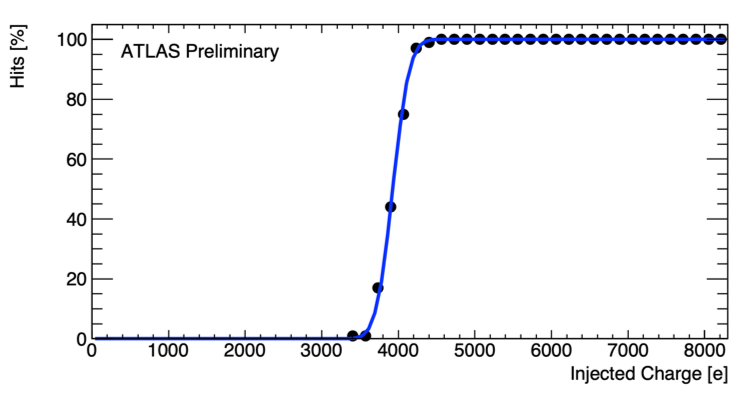
\includegraphics[height=7cm,keepaspectratio]{threshold.png}
  \caption[検出効率と試験電荷の関係]{検出効率と試験電荷の関係 \cite{calibsoft}。検出効率が 50\% となる試験電荷の値がThresholdであり、検出効率が30\%と 70\% となる試験電荷の幅がノイズである。}
  \label{fig:threshold}
\end{figure}


%------------------------------------------------------------------------------------------------------------------------
\subsubsection{ToTスキャン}
\label{sec:totscan}
%------------------------------------------------------------------------------------------------------------------------
ToTスキャンでは、一定の試験電荷を各ピクセルに100回入射させ、その試験電荷に対するToTの値の測定を行う。各ピクセルから得られるToTの値はデジタル値であるため整数値であるが、100回のスキャンの平均値をある試験電荷に対するToTとするため、この値は小数値を取り得る。


%------------------------------------------------------------------------------------------------------------------------
\subsection{電荷較正}
\label{sec:calibration}
%------------------------------------------------------------------------------------------------------------------------
\ref{sec:ASIC}で示した様に、ToTは荷電粒子がシリコンセンサーに落とす電荷量$Q$に比例すると予想される。しかし、実際には三角波の傾きが完全に一致しないこと等による二次な効果により、ToTと電荷量は直線ではなくなり\eref{eq:calibration}の様に表される。
\begin{equation}
  \label{eq:calibration}
  \mathrm{ToT} = p_0\frac{p_1 + Q}{p_2 + Q}
\end{equation}
\eref{eq:calibration}に示した3つのパラメータを求めるために、電荷量を変えながら試験電荷を入射し、ToTの較正を行う。電荷較正は各ピクセルに対してパラメータを求めるのではなく、FEチップごとに一律の値を用いる。そのため、ToTスキャンから得られたピクセルごとのToTの平均値を用いてFEチップに対する電荷較正を行う。

IBLについてはToTの出力が4bitと少ないことから、RUN3からは\eref{eq:calibration}によるフィッティングは行わず、ToTの値と試験電荷の値をルックアップテーブルを用いて変換を行う。本研究では電荷較正手法について取り扱うため、以下ではピクセル検出器についてのみについて述べる。

%------------------------------------------------------------------------------------------------------------------------
\section{電荷較正結果の履歴}
\label{sec:probrem}
%------------------------------------------------------------------------------------------------------------------------
Thresholdのチューニングや電荷較正を行った後、それらに関する情報はCERNに設置されているデータベース\cite{pixeldb}に保存する必要がある。このデータベースでは電荷較正に関する情報や検出器の配置や温度等のDCS(Data Control System)情報、さらにトリガー情報等を保管する。これらの情報は、測定におけるイベント選別やモンテカルロシミュレーションのためのイベント作成等に用いられる。

ThresholdスキャンおよびToTスキャンは各ピクセルごとの値を出力するが、データベースへはあるFEチップにおけるThresholdの平均値およびToTの平均値を用いた電荷較正式(\ref{eq:calibration})のパラメータのみを登録する。また、各ピクセルの大部分は\tref{tab:asicsiyou}に示した構造をしているが、FEチップの境界付近では不感領域をなるべく少なくするために、構造の異なったピクセルを配置する。FE-I3の境界付近におけるピクセルの構造を\fref{fig:pixeltypes}に示す。\tref{tab:asicsiyou}に示した通常のピクセルのことをnormalピクセル(図中の青の領域)と呼び、黄色の領域のピクセルをlongピクセル、赤色の領域をgangedピクセルと呼ぶ。longピクセルは$50\times 600\ \si{\micro m^2}$であり、長方形の一辺の長さがnormalピクセルの1.5倍となっている。また、gangedピクセルはnormalピクセル2つをワイヤーで接続した構造をしている。このような構造の違いから、ノイズ等の値が異なる値になるため、データベースへはそれぞれの値をアップロードする。

\begin{figure}[tbp]
  \centering
  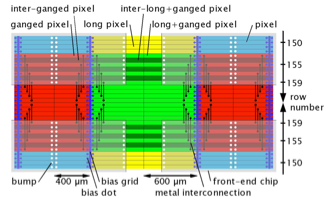
\includegraphics[height=6cm,keepaspectratio]{pixeltypes.png}
  \caption[ピクセルモジュールのFEチップ境界付近のピクセルタイプ]{ピクセルモジュールのFEチップ境界付近のピクセルタイプ \cite{pixeltypes}。}
  \label{fig:pixeltypes}
\end{figure}

データベースに登録する情報を以下に示す。
\begin{itemize}
  \item Thresholdの平均値
  \item Thresholdの分散
  \item Thresholdのノイズ
  \item In-time threshold
  \item 電荷較正式(\ref{eq:calibration})における3つのパラメータ
  \item 電荷較正におけるフィッティングの誤差
\end{itemize}




\newpage
